\section{Elkies' Small Values}\label{sec:targets}

Elkies~\cite{Elkies1996} found fractions, ups and tinies in chess endgames on the ordinary board. The flat census
lets us ask which smaller values of this kind occur with at most six pawns, and where. Each halving is one more
step: $1/8=\game{0}{1/4}$, $1/16=\game{0}{1/8}$ and $1/32=\game{0}{1/16}$. Up-second and the tinies were
defined in Section~\ref{sec:rules}; adding $\star$ to up-second gives $\upsec\star=\game{0,\star}{{\downarrow}}$.

\begin{table}[!t]
\caption{Elkies' Targets in the Flat Census}
\label{tab:targets}
\centering
\begin{tabular}{@{}llcc@{}}
\toprule
Target & Form & Textbook & E.p.-aware \\
\midrule
$1/8$ & $\game{0}{1/4}$ & $13$ & $9$ \\
$1/16$ & $\game{0}{1/8}$ & $3$ & $2$ \\
$1/32$ & $\game{0}{1/16}$ & $1$ & $0$ \\
$\upsec$ & $\game{0}{{\downarrow}\star}$ & $5$ & $2$ \\
$\upsec\star$ & $\game{0,\star}{{\downarrow}}$ & $10$ & $10$ \\
$\tinyg{1}$ & $\ggame{0}{0\mid -1}$ & $13$ & $16$ \\
$\tinyg{x}$, $x\notin\mathbb{Z}$ & $\ggame{0}{0\mid -x}$ & $0$ & $0$ \\
\bottomrule
\end{tabular}

\smallskip
\parbox{\columnwidth}{\footnotesize Number of positions of each exact value; flat boards of one to four files,
at most six pawns, count rule, en passant on. Every counted identity was confirmed by an independent solver
\lab{C2}.}
\end{table}

Table~\ref{tab:targets} counts the positions of each target under both passed-pawn tests. For every counted
position $G$ and target $T$, an independent C solver checked that $G-T=0$. The e.p.-aware test thins out the
smallest numbers: $1/32$ disappears and $1/16$ drops to two positions. Up-second falls from five positions to two, while $\upsec\star$ is untouched and $\tinyg{1}$ rises from $13$ to $16$.

\begin{figure*}[!t]
\centering
\begin{subfigure}[b]{0.3\textwidth}\centering
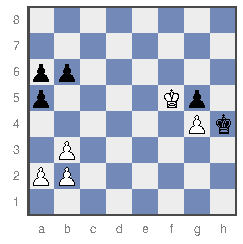
\includegraphics[width=1.62in]{figures/eighth.pdf}
\caption{}
\end{subfigure}\hfil
\begin{subfigure}[b]{0.3\textwidth}\centering
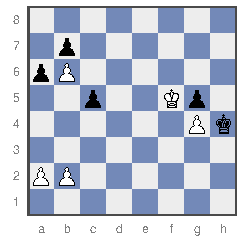
\includegraphics[width=1.62in]{figures/upsecstar.pdf}
\caption{}
\end{subfigure}\hfil
\begin{subfigure}[b]{0.3\textwidth}\centering
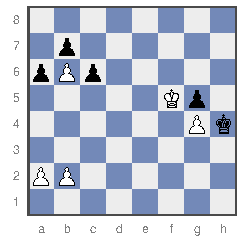
\includegraphics[width=1.62in]{figures/tiny1.pdf}
\caption{}
\end{subfigure}
\caption{Elkies' small values beside the tr\'ebuchet (white Kf5 and g4, black Kh4 and g5), each a legal
10-man position (ordinary board). (a)~$1/8$: white a2, b2, b3 against black a5, a6, b6. (b)~$\upsec\star$:
white a2, b2, b6 against black a6, b7, c5. (c)~$\tinyg{1}$: white a2, b2, b6 against black a6, b7, c6.}
\label{fig:eighth}
\end{figure*}

\subsection{An Eighth That Can Happen in a Game}

\begin{theorem}[\lab{C2}]\label{thm:eighth}
In the pawn model, white a2, b2, b3 against black a5, a6, b6 has value exactly $1/8$. This holds in all nine
settings (the three race rules, each with en passant off, with the textbook test and with the e.p.-aware test)
and for every assignment of outcomes to its race positions.
\end{theorem}

So this $1/8$ does not depend on how races are settled at all. A third, separately written solver agrees in all
nine settings.

Let's see why (Fig.~\ref{fig:eighth}(a)). If white (Left) moves first, a2--a4 locks the a-file and leaves the
zero game. The quieter a2--a3 only reaches $\star$, a reversible move, since black answers it back to $0$. The
move b3--b4 is bad: black answers to $-3$. If black (Right) moves first, b6--b5 leaves $1/4$, and a5--a4 is bad.
Thus $G=\game{0}{1/4}=1/8$.

This pawn structure can arise in a real game. From the starting position, c2$\times$b3, a7--a5, b7$\times$a6 and c7$\times$b6
produce it. Its mirror image, white a2, a3, b2 against black a6, b5, b6, has the same value but cannot arise:
the pawn on a3 could only have come from b2, which is still occupied. Beside the tr\'ebuchet, the $1/8$ becomes
the legal 10-man position of Fig.~\ref{fig:eighth}(a). Whether it keeps its value with real kings is the subject
of Section~\ref{sec:real}.

\subsection{Up-Second Star and Tiny 1}
White a2, b2, b6 against black a6, b7, c5 (Fig.~\ref{fig:eighth}(b)) is $\upsec\star$ in all nine settings
\lab{C2}. If white moves first, a2--a4 leaves $0$ and a2--a3 leaves $\star$. If black moves first, a6--a5 leaves
${\downarrow}$. Thus $G=\game{0,\star}{{\downarrow}}=\upsec\star$.

Now move the black c-pawn back to c6 (Fig.~\ref{fig:eighth}(c)). If white moves first, a2--a3 leaves $0$. If
black moves first, a6--a5 leaves $-1/2\pm1/2=\game{0}{-1}$. Black's other move, c6--c5, reaches exactly the
$\upsec\star$ position above, and it is dominated, since $\game{0}{-1}\le\upsec\star$. Thus
$G=\ggame{0}{0\mid -1}=\tinyg{1}$ with en passant on, under every race rule \lab{C2}. Unlike the Tiny~1 of
Section~\ref{sec:basic}, which lives on the a- and h-files across the seam, this one fits on the ordinary board
beside the tr\'ebuchet.

\subsection{Two Textbook Results That Do Not Survive}
Under the textbook test we had found a $1/8$ at white a2, b2, d2 against black a5, c4, d7, which we singled out
as reachable, and an exact $\upsec$ at white a3, c5, d4 against black a7, b7, d7. Under the e.p.-aware test the
first is worth $-3/2\pm3/2$ and the second $\game{3/4}{{\downarrow}\star}$. The two tests differ only just after a
double step that the opponent may still take en passant, so both values rested on such a pawn being counted as
passed. This is why we ask for values that, like Theorem~\ref{thm:eighth}, hold in all nine settings.
